\subsection{面图形的绘制}

\subsubsection{单位圆,单位矩形}
Asymptote 预先定义了很多画基本图形的函数,经常调用的有:\\
\begin{description}
  \item[box] (矩形的左下角, 矩形的右上角);
  \item[ellipse] (椭圆的中心, 水平方向的轴长, 竖直方向的轴长);
  \item[drawline] (直线的第一个点, 直线上的第二个点);
  \item[unitcircle,unitcircle3] 单位圆
  \item[unitsquare,unitsquare3] 单位正方形
  \item[unitsphere] 单位球 - - 3D
  \item[unitbox,unitcube] 正方体 - - 3D
  \item[旋转体函数] 如unitsphere, unitcone, unitcylinder, unitsolidcone,%
  unithemisphere, unitfrustum(real t1, real t2) 等等。
  \item[polygon(n)] 正多边形

\end{description}

  \lstinputlisting{body/asycode/surface.asy}


\begin{figure}[htbp]
  % Requires \usepackage{graphicx}
  \centering
  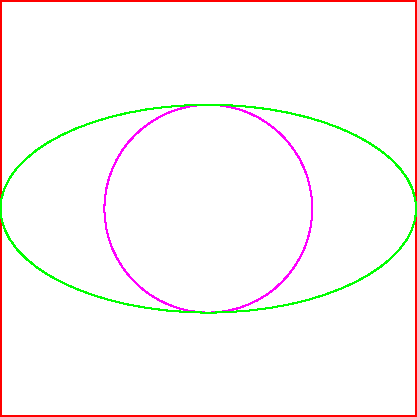
\includegraphics[width=8cm]{body/asycode/surface.pdf}\\
  \caption{对应曲线}\label{surface}
\end{figure}

\subsubsection{封闭曲面}
\clearpage
